\documentclass{article}
\usepackage[margin=0.6in]{geometry}
\usepackage[utf8]{inputenc}
\usepackage{physics}
\usepackage{graphicx}
\usepackage{siunitx}
\usepackage{amsmath}
\usepackage{amssymb}
\usepackage[dvipsnames]{xcolor}
\usepackage[sort&compress]{natbib}
\usepackage{bm}
\usepackage{url}
\usepackage{hyperref}
\usepackage{parskip}
\usepackage{lineno}
\usepackage{float}
\usepackage{gensymb}
\usepackage{appendix}
\linenumbers

\setlength\parindent{0pt}
\renewcommand{\baselinestretch}{1.5}

\newcommand{\TODO}[1]{\todo[inline,backgroundcolor=red!25,bordercolor=red]{#1}}
\newcommand{\alan}[2][]{\todo[color=green, #1]{\textbf{Alan}: #2}}
\newcommand{\henri}[2][]{\todo[color=orange, #1]{\textbf{Henri}: #2}}
\usepackage[obeyFinal,textsize=footnotesize]{todonotes}


\usepackage{authblk}

\title{A multi-thronged and responsive policy process for climate decision-making}
\author[1,2]{Henri F. Drake\textsuperscript{*}}
\author[1]{Ron Rivest}
\author[1]{Alan Edelman}
\author[1]{John Deutch}
\affil[1]{Massachusetts Institute of Technology, Cambridge, MA, USA}
\affil[2]{Woods Hole Oceanographic Institution, Woods Hole, MA, USA}

\date{}             %% if you don't need date to appear
\setcounter{Maxaffil}{0}
\renewcommand\Affilfont{\itshape\small}

\begin{document}
\maketitle

\section{Background and motivation}

Coming soon.

% Ever since climate scientists began understanding how anthropogenic emissions of greenhouse gases and aerosols have unintentionally altered Earth's climate \citep{manabe1967thermal, schneider_carbon_1975, broecker_climatic_1975}, they have speculated about the intentional manipulation of such mechanisms for climate control \citep[][and references therein]{kellogg_climate_1974}.

% Using carbon geoengineering and solar geoengineering to assist mitigation in controlling climate, since ambitious climate goals of 1.5 deg (and maybe even 2 deg) are slipping out of reach.

% Review of the four basic climate controls.

% Joint optimization.

% Review of IAMs, CBA and CEA, and limitations.

% Recognizing some of the above limitations of IAMs, \cite{lempert_when_1996} propose an ``adaptive strategy" in which policy-makers wait to deploy aggressive abatement until either 1) damages overshoot a pre-determined threshold or 2) abatement costs decrease faster than a pre-determined rate. \cite{lempert_when_1996} show that, in the face of large parameter uncertainties, the expected benefits of even this simple adaptive strategy dwarf those of any individual deterministic optimal trajectory, which only performs well in a local region of a vast parameter space. While this ad-hoc approach highlights the potential utility of a sequential strategy, it permits potentially catastrophic overshoots of climate goals and is not extendable to a higher-dimensional framework in which there are multiple climate controls to choose from.

% Role of models in climate policy

% In this paper, we propose an alternative ``responsive policy process", which combines the flexibility of an sequential decision-making approach \citep[e.g.][]{hammitt_sequential-decision_1992, lempert_when_1996} with the rigor of formal optimization methods.

% % , either by afforestation, soil carbon sequestration, direct air capture, bio-energy and carbon capture and sequestration, or enhanced weathering (see reviews of \citealt{minx_negative_2018, fuss_negative_2018}).


% More coming soon.

% \alan[inline]{Nice to mention En-Roads, and mention that
% it also seeks to raise consciousness }

\section{MARGO: An idealized model of optimally-controlled climate change}

The \textbf{MARGO} model consists of a physical energy balance model of Earth's climate, an idealized socio-economic model of climate damages and controls:
\begin{center}
\begin{tabular}{l}
\textbf{M}itigation of greenhouse gas emissions, \\
\textbf{A}daptation to climate impacts, \\
\textbf{R}emoval of carbon dioxide, \\
\textbf{G}eoengineering by radiation management,
\end{tabular}
\end{center}
and a modular, fast, and customizable \textbf{O}ptimization model with several options of objective functions and constraints. 
\henri[inline]{I am open to other naming options, but do not like MARS or ARMS (Adaptation Removal Mitigation Solar-geoengineering), as it sounds fairly military to me... I like MARGO because it places the four technologies roughly in their order of socio-technological readiness and because it is both memorable and easy to pronounce.}

Each of the climate controls acts, in its own distinct way, to reduce the damages caused by a changing climate but also carry their own deployment costs (including research and development costs, infrastructure costs, political costs, costs of unintended damages, etc). The model is designed to include key features of climate physics, economics, and policy as concisely as possible and in ways qualitatively consistent with both fundamental theory and more comprehensive models. We aim to construct a model which yields fundamental insights into the optimal management of climate change but is significantly more accessible, transparent, flexible, and computationally inexpensive than conventional models. The cost of the models' extreme simplicity is that its results should only be interpreted as qualitative insights, not quantitative predictions.

The model is developed in open source using the Julia programming language \citep{bezanson_julia:_2017} at \url{github.com/hdrake/OptimizeClimate} (Drake et al., 2020). The parameter values used throughout the paper are set to the defaults in Tables \ref{tab.parameters} and \ref{tab.controls}, except where explicitly stated otherwise, and are justified in Section 1 of the Supplementary Information. In Section 2 of the Supplementary Information, we show that by tweaking just a handful of these default parameter values, the model replicates the qualitative results of studies ranging from analytical control theory analysis of solar-geoengineering deployments \citep{soldatenko_optimal_2018} to numerical optimizations of mitigation, carbon dioxide removal, and solar geo-engineering deployments in DICE, a commonly used Integrated Assessment Model \citep{belaia_optimal_2019}.

\subsection{CO$_{2}$ concentrations: baseline emissions, emissions reductions, and negative emissions}

In the absence of climate policy, we assume CO$_{2}$ concentrations in the model start at present values of $c_{0} \equiv c(t_{0})$ in $t_{0}=2020$ and increase according to a baseline emissions scenario $q(t)$. The baseline concentrations are given by the accumulation of emissions in the atmosphere,
\begin{equation}
c(t) = c_{0} + \int_{t'=t_{0}}^{t} rq(t') \text{ d}t',
\end{equation}
where $r \approx 40\%$ is the fraction of emissions which remain in the atmosphere, net of uptake by the terrestrial biosphere and the ocean \citep{solomon_irreversible_2009}, and $rq(t)$ are the \textit{effective emissions} that contribute to planetary warming via the greenhouse effect. The model currently has no explicit carbon cycle but in the future will include an idealized dynamic ocean carbon cycle \citep[e.g.][]{glotter_simple_2014}, which captures both the initial linear uptake of carbon by the ocean and non-linear feedbacks due to the ocean's limited chemical buffering capacity. While we here only explicitly model CO$_{2}$ effects, other greenhouse gases may be approximated by forcing the model with the CO$_{2}$ concentrations that result in the equivalent global-mean forcing from all greenhouse gases, referred to as carbon dioxide-equivalent concentrations CO$_{2e}$. The radiative effects of aerosols (and other minor anthropogenic effects) are similarly bundled into CO$_{2e}$ but could instead be prescribed as additional time-dependent global-mean forcing terms, with associated damages (e.g. the negative health effects of airborne particulate matter) which could in turn be reduced by air pollution abatement policies \citep{thompson_systems_2014}.

For simplicity, we calibrate our baseline effective emissions to the high-end no-climate-policy Representative Concentration Pathway (RCP) 8.5, which results in $\SI{8.5}{W m^{-2}}$ of radiative forcing by 2100 relative to preindustrial levels, mostly due to greenhouse gas emissions from rampant fossil fuel consumption \citep{riahi_scenarios_2007}. We approximate the RCP8.5 emissions by the continuous and piecewise linear function:
\begin{equation}
    q(t) = 
    \begin{cases}
        q_{0}(1 + 2\frac{2100-t}{2100-2020}) &\mbox{if } t \le 2100 \\
        3q_{0}\frac{2150-t}{2150-2100} &\mbox{if } 2100 < t \le 2150 \\
        0 &\mbox{if } 2150 < t
    \end{cases},\label{eq.baseline_emissions}
\end{equation}
in which CO$_{2e}$ emissions increase linearly from a present-day value $q_{0} = \SI{10}{ppm\, yr^{-1}}$ ($\SI{50}{GtCO_{2e}\, yr^{-1}}$) to a maximum of $3q_{0} = \SI{30}{ppm\, yr^{-1}}$ in $2100$ and then decrease linearly to zero by $2150$ (Figure \ref{fig.temp_and_carbon}a). These effective emissions $rq(t)$ result in CO$_{2e}$ concentrations of about $\SI{1400}{ppm}$ and a corresponding anthropogenic radiative forcing of $\SI{8.5}{W\, m^{-2}}$ by $2150$, relative to preindustrial levels (see below).

CO$_{2}$ emissions reductions are parameterized by the fractional \textbf{M}itigation of annual emissions $M(t) \in [0,1]$ such that the net annual emissions become $q(1-M(t))$. In acknowledgement of existing mitigation policies that make our current trajectory diverge from RCP8.5 \citep{hausfather_emissions_2020}, we assume modest present day mitigation of $M(t_{0}) = \SI{5}{\%}$.

CO$_{2}$ \textbf{R}emoval is parameterized by the fraction $R(t) \in [0,1]$ of the baseline emissions $q_{0}$ in $2020$ that are sequestered from the atmosphere in a given year. The CO$_{2}$ concentrations in a given year are thus given by (Figure \ref{fig.temp_and_carbon}b):
\begin{equation}
    c_{M, R}(t) = c_{0} + \int_{t'=t_{0}}^{t} r(1-M(t'))q(t') - R(t')q_{0} \text{ d}t'\label{eq-CO2-conc},
\end{equation}
where $c_{0} \equiv c(t_{0}) \approx \SI{460}{ppm}$ is roughly the present CO$_{2e}$ concentration. Figures \ref{fig.temp_and_carbon}a,b show the effective CO$_{2e}$ emissions and concentrations, respectively, for both the baseline scenario and an example of an optimally-controlled scenario.

The anomalous heat trapped by CO$_{2}$, hereafter ``radiative forcing", is theoretically and empirically found to be a logarithmic function of CO$_{2}$ concentrations
\begin{equation}
    F(t) = a \ln(\frac{c(t)}{c_{0}}),
\end{equation}
relative to $t_{0} = 2020$ and where $a \approx \SI{4.97}{W m^{-2}}$ \citep{geoffroy_transient_2012}. The controlled greenhouse forcing is similarly given by:
\begin{equation}
    F_{M, R}(t) = a \ln(\frac{c_{M, R}(t)}{c_{0}}).
\end{equation}

The controlled greenhouse radiative forcing $F_{M, R}$ is (optionally) partially offset by Solar-\textbf{G}eoengineering measures, which reduce the rate at which solar radiation is absorbed by the surface and consequently impose a negative radiative forcing
\begin{equation}
F_{G}(t) \equiv -G(t)F(t \rightarrow \infty),
\end{equation}
determined by the fraction $G(t) \in [0,1]$ of the ultimate greenhouse forcing  $F(t \rightarrow \infty) = \SI{8.5}{W\, m^{-2}}$ that is offset by controlling solar radiation. The controlled net radiative forcing is thus given by:
\begin{equation}
    F_{M, R, G}(t) = F_{M, R}(t) + F_{G}(t).
\end{equation}

\begin{figure}[htb!]
\noindent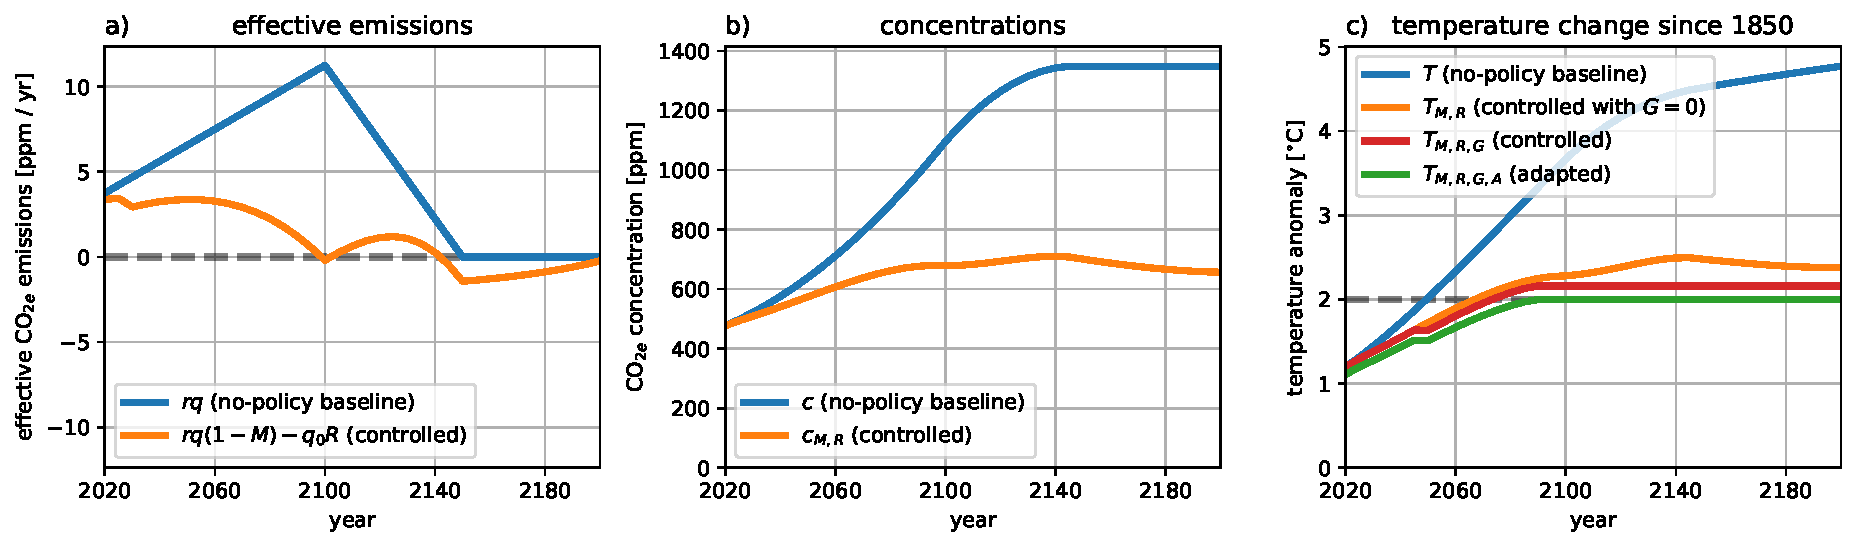
\includegraphics[width=1.0\textwidth]{figures/default-temp_carbon_and_temperatures.pdf}
\centering
\caption{Baseline (blue) and optimally-controlled (orange) a) effective CO$_{2e}$ emissions, b) CO$_{2e}$ concentrations, and c) temperature anomaly relative to preindustrial from cost-effectiveness analysis (see Section \ref{sec.cost-effectivness}). Panel c) shows the optimal temperature change that would occur: in a baseline scenario (blue); with just emissions \textbf{M}itigation and carbon dioxide \textbf{R}emoval (orange); with \textbf{M}itigation, \textbf{R}emoval, and solar-\textbf{G}eoengineering (red); and as an ``adapted temperature" (eq. \ref{eq.adapted_temperature}) with \textbf{A}daptation measures also taken into account. The dashed grey line marks the threshold adapted temperature of $T^{\star} = \SI{2}{\celsius}$ to be avoided.}
\label{fig.temp_and_carbon}
\end{figure}

\subsection{Temperature response to CO$_{2}$ forcing}
The evolution of the global-mean near-surface temperature anomaly (relative to the initial time $t_{0} = 2020$) is determined by the two-box linear energy balance model \citep[e.g][]{gregory_vertical_2000, held_probing_2010}:
\begin{gather}
    C_{U} \dv{T}{t} = -B T - \kappa( T - T_{D}) + F(t), \label{eq.upper_ocean}
    \\
    C_{D} \dv{T_{D}}{t} = \kappa (T - T_{D}),\label{eq.deep_ocean}
\end{gather}
where (\ref{eq.upper_ocean}) represents the upper ocean with average temperature anomaly $T$, and (\ref{eq.deep_ocean}) represents the deep ocean with an average temperature $T_{D}$. The near-surface atmosphere exchanges heat rapidly with the upper ocean and thus the global-mean near-surface air temperature is also given by $T$. The physical model parameters are: the upper ocean heat capacity $C_{U}$ (including a negligible contribution $C_{A} \ll C_{U}$ from the atmosphere); the deep ocean heat capacity $C_{D}$; the climate feedback parameter $B$; the ocean mixing rate $\kappa$; and $F(t)$ the anomalous anthropogenic radiative forcing. The radiative forcing and temperature anomalies at $t_{0} = 2020$ relative to preindustrial are $F(t_{0}) - F(t_{\text{pre}}) = \SI{2.5}{W\, m^{-2}}$ and $T_{0} \equiv T(t_{0}) - T(t_{\text{pre}}) = \SI{1.1}{K}$, where we set $F_{0} \equiv F(t_{0}) = \SI{0}{W\, m^{-2}}$ and $T(t_{\text{pre}}) = \SI{0}{K}$ for convenience.

Since, by construction, the anthropogenic forcing $F(t)$ varies on timescales longer than the fast relaxation timescale $\tau_{U} = C_{U}/(B + \kappa)$, we can ignore the time-dependence in the upper ocean and approximate
\begin{equation}
    T \approx \frac{F+\kappa T_{D}}{B + \kappa},
    \label{eq.shallow_approx}
\end{equation}
where the evolution of the deep ocean
\begin{equation}
    C_{D} \dv{T_{D}}{t} \approx - \frac{B \kappa}{B + \kappa} T_{D} + \frac{\kappa}{B + \kappa} F
    \label{eq.deep_ode}
\end{equation}
occurs on a slower timescale $\tau_{D} \equiv \dfrac{C_{D}}{B} \dfrac{B + \kappa}{\kappa}$ \citep{held_probing_2010}. Plugging the exact solution to (\ref{eq.deep_ode}) into (\ref{eq.shallow_approx}) gives the closed solution
\begin{equation}
    T(t) - T_{0} = \frac{F(t)}{B + \kappa} + \frac{\kappa}{B} \frac{1}{(B+\kappa)} \int_{t_{0}}^{t} \frac{ e^{-(t-t')/\tau_{D}}}{\tau_{D}} F(t') \, \text{d}t'.\label{eq.baseline_temperature}
\end{equation}
The evolution of the controlled temperature anomaly (Figure \ref{fig.temp_and_carbon}c)
\begin{equation}
    T_{M,R,G}(t) - T_{0} =  \frac{F_{M,R,G}(t)}{B + \kappa} + \frac{\kappa}{B} \frac{1}{(B+\kappa)} \int_{t_{0}}^{t} \frac{ e^{-(t-t')/\tau_{D}}}{\tau_{D}} F_{M,R,G}(t') \, \text{d}t'\label{eq.temperature}
\end{equation}
is thus driven by the controlled net radiative forcing $F_{M,R,G}$.

We identify the first term on the right hand side of (\ref{eq.baseline_temperature}) and (\ref{eq.temperature}) as the transient climate response \citep{gregory_transient_2008}, which dominates for $t-t_{0} \ll \tau_{D}$, while the second term is a slower ``recalcitrant" response due to a weakening of ocean heat uptake as the deep ocean comes to equilibrium with the upper ocean \citep{held_probing_2010}. While the contribution of the recalcitrant component to historical warming is thought to be small, it contributes significantly to 21st century and future warming \citep{gregory_transient_2008,held_probing_2010}. If the instantaneous radiative forcing vanishes, as in the case of either complete decarbonization or strong solar geoengineering, or remains constant, the recalcitrant component is the only remaining cause of temperature change (Figure \ref{fig.temp_and_carbon}c, see also \citealt{gregory_transient_2008, held_probing_2010, lickley_time_2019}).

The behavior of the model on short and long timescales is illustrated by applying it to the canonical climate change experiment in which CO$_{2}$ concentrations increase at 1\% per year until doubling. The temperature anomaly first rapidly increases until it reaches the Transient Climate Sensitivity $TCS = \dfrac{F_{2\times}}{B + \kappa}$ around the time of doubling $t=t_{2\times}$, with $t_{2\times} - t_{0} \ll \tau_{D}$ and $F_{2\times} = \alpha \ln(2)$, and then gradually asymptotes to the Equilibrium Climate Sensitivity $ECS = \dfrac{F_{2\times}}{B} > TCS$ on a much longer timescale $t-t_{0} \gg \tau_{D}$.

\subsection{Climate damages}

Annual climate damages are assumed to quadratic, $D(t) = \beta T(t)^{2}$, such that successive temperature increases are increasingly damaging, based on empirical estimates of damages which range from linear to cubic functions of absolute global-mean temperature change relative to preindustrial \citep{stern_economics_2007}. The default value of the damage parameter $\beta \equiv \tilde{\beta} E(t)$ is chosen to be roughly similar to the DICE model for low levels of warming \citep{nordhaus2013dice}, resulting in damages of $2\%$ of the Global World Product (GWP) $E(t)$ at \SI{3}{\celsius}, or $\tilde{\beta} = \dfrac{\SI{2}{\%}}{\SI{9}{\celsius^{2}}}$. Economic growth is insensitive to policy changes or climate damages at leading order in Integrated Assessment Models such as DICE \citep[see Figure 3 of][]{nordhaus2013dice}, although this may be due to an underestimation of climate damages and their impacts on growth \citep{burke_global_2015, glanemann_paris_2020}. Thus, for simplicity, we here ignore economic feedbacks and assume the GWP, $E(t) = E_{0}(1 + \gamma)^{(t-t_{0})}$, is determined by a fixed exogenous economic growth rate $\gamma$.

\textbf{A}daptation to climate change impacts (e.g. building sea walls, installing air conditioning units, planting climate-resilient crops) is parameterized by reducing annual damages by a fraction $A(t) \in [0, 1/3]$, such that the total controlled damages are:
\begin{equation}
    D_{M, R, G, A} = \beta (T_{M, R, G}(t))^{2} \; (1-A(t)).
\end{equation}
Although adaptation does not affect the planetary temperature directly, it is useful to consider an ``adapted temperature" $T_{M,R,G,A}$ which yields damages equivalent to the fully-controlled damages $\beta (T_{M,R,G,A})^{2} = \beta (T_{M,R,G})^{2} (1-A)$, given by
\begin{equation}
    T_{M,R,G,A} \equiv T_{M,R,G} \sqrt{(1-A)}.\label{eq.adapted_temperature}
\end{equation}
In Figure \ref{fig.temp_and_carbon}, for example, while the controlled temperature $T_{M,R,G}$ slightly overshoots the $\SI{2}{\celsius}$ warming threshold, the ``adapted temperature" $T_{M,R,G,A}$ remains below the threshold.

\subsection{Control costs}

The annual cost of deploying climate controls is given by
\begin{equation}
    \mathcal{C}_{M, R, G, A}(t) = \sum_{\alpha \in \mathcal{A}} \mathcal{C}_{\alpha} f^{(\alpha)}(\alpha(t)),
\end{equation}
where $\mathcal{A} = \{M, A, R, G \}$ is the set of climate controls, $\mathcal{C}_{\alpha}$ is the reference cost of each climate control, and $f^{(\alpha)}(\alpha)$ is a function that determines how the deployment cost increases as a function of fractional deployment. The reference cost $\mathcal{C}_{\alpha}$ corresponds to the hypothetical cost of full deployment of that control (e.g. $\mathcal{C}_{M}$ is the annual cost of fully decarbonizing society). However, the reference costs may be more usefully tuned based on a smaller deployment threshold, for which cost estimates are likely to be more accurate and reflective of plausible near-future deployment fractions.

We will here assume the reference costs of mitigation $\mathcal{C}_{M}$, removal $\mathcal{C}_{R}$, and adaptation $\mathcal{C}_{A}$ are fixed in time and reflect the required investments in abatement measures. In contrast, we argue that the reference cost of geoengineering $\mathcal{C}_{G}$ is dominated by the damages due to unintended side effects rather than the direct costs of deployment, which are thought to be relatively small \citep{mcclellan_cost_2012}. The reference cost of geoengineering is thus given by $\mathcal{C}_{G}(t) = \tilde{\mathcal{C}}_{G} E(t)$, where $\tilde{\mathcal{C}}_{G}$ is the damage due to deploying $-F_{\infty} \equiv -F(t \rightarrow \infty) = \SI{-8.5}{W m^{-2}}$ worth of solar radiation management, as a fraction of the exogenous GWP, $E(t)$. In the face of deep uncertainties about the climate impacts of large-scale solar geoengineering \citep{irvine_towards_2017}, we make the conservative assumption that the unintended damages of solar geoengineering are as large as the uncontrolled damages due to an equivalent amount of CO$_{2e}$ forcing \citep[as in][]{goes_economics_2011, belaia_optimal_2019}, i.e. $\tilde{\mathcal{C}}_{G} \equiv \tilde{\beta} (F_{\infty}/B)^{2} \approx \SI{4.6}{\%}$, where $F_{\infty}/B$ is the equilibrium temperature response to a fixed radiative forcing of $F_{\infty} = \SI{8.5}{W m^{-2}}$.

We do not include learning effects beyond their possible influence in setting the reference costs $\mathcal{C}_{\alpha}$ or the shape of the deployment cost functions $f^{(\alpha)}(\alpha) = \alpha^{p_{\alpha}}$. Here, we will focus on the commonly-used medium deployment cost scenario $f(\alpha) = \alpha^{2}$ ($p_{\alpha} = 2$ for all $\alpha \in \mathcal{A}$), which has the following interpretable properties: 
\begin{itemize}
    \item $\left. \dv{f}{\alpha}\right|_{\alpha=0} = 0$ (initial marginal deployment is effectively free)
    \item $f(1) = 1$ (full deployment costs $\mathcal{C}_{\alpha}$), and
    \item $\dv[2]{f}{\alpha} > 0$ (convex, such that deployment gets progressively more and more expensive).
\end{itemize}

\subsection{Optimization Methods}

We use the Interior Point Optimizer (\citealt{wachter_implementation_2006}, \url{https://github.com/coin-or/Ipopt}), an open source software package for large-scale nonlinear optimization, to minimize objective functions representing benefits and costs to society subject to assumed policy constraints, as described in Section \ref{sec.policy_frameworks}. In practice, the control variables $\alpha \in \mathcal{A} = \{ M, R, G, A\}$ are discretized into $N = (t_{f} - t_{0}) / \delta t$ timesteps (default $\delta t = \SI{5}{years}$) resulting in a $4N$-dimensional optimization problem. In the default (deterministic and convex) configuration, the model takes only $\mathcal{O}(\SI{10}{ms})$ to solve after just-in-time compiling and effectively provides user feedback in real time, making it amenable to our forthcoming interactive web application (e.g. following the lead of the impactful \href{https://en-roads.climateinteractive.org/scenario.html?v=2.7.11}{En-ROADS} model, \citealt{siegel2018roads}) and future extension of the model to high-dimensional stochastic optimization.

\section{Climate change policy frameworks}\label{sec.policy_frameworks}

In contrast to conventional Integrated Assessment Models, which follow classic economic theories of optimal economic growth and solve for the maximal welfare based on the discounted utility of consumption, we here treat economic growth as exogenous (ignoring economy-policy-climate feedbacks) and simply aim to minimize the costs– and maximize the benefits– of deploying climate change controls, subject to constraints from policy goals.

In Section \ref{sec.cost_benefit}, we describe a cost-benefit analysis approach which finds the trajectories of control deployments that optimize trade-offs between the costs of deploying climate controls and the benefits of these controls in terms of avoided climate damages. The cost-benefit approach depends strongly on the magnitude of the poorly-constrained damage function $D(T)$, which is thought to be under-estimated by conventional bottom-up approaches \citep{ackerman_limitations_2009}. Thus, in Section \ref{sec.cost-effectivness} we also explore an alternative scenario in which we instead impose an upper bound on permissible climate damages, or temperatures (as in the 2015 United Nations Paris Agreement on Climate Change), and find the lowest cost climate control trajectories which still satisfy this constraint.

\paragraph{Policy and technology readiness constraints.} For each control $\alpha \in \mathcal{A} = \{ M, R, G, A\}$, we assert a maximum deployment rate
\begin{equation}
    \abs{\dv{\alpha}{t}} \le \dot{\alpha},
\end{equation}
to forbid implausibly aggressive deployment and phase-out scenarios, and a readiness condition
\begin{equation}
    \alpha(t < t_{\alpha}) = \alpha_{0},
\end{equation} where typically $\alpha_{0} = 0$ and $t_{\alpha} \ge t_{0}$ is the earliest time at which the control is ``ready" to be deployed. In particular, in the default configuration we set $t_{R} = 2030$ and $t_{G} = 2050$ because these socio-technological systems do not yet exist at a climatically-significant scale \citep{minx_negative_2018, flegal_solar_2019}. Additionally, we interpret adaptation deployment costs as buying insurance against future damages at a fixed annual rate $\mathcal{C}_{A} f^{(A)}(A)$, with $\dot{A} = 0$, which can be increased or decreased upon re-evaluation at a later date (see Section \ref{sec.reactive}).

\paragraph{Discount rates.} A common economic assumption is that society discounts future costs and benefits relative to the present by a multiplicative discount factor $(1 + \rho)^{-(t-t_{0})}$, determined by the utility discount rate $\rho$ \citep[e.g. see reviews in][]{broome_discounting_1994, stern_economics_2007}. Ethical justifications for applying a non-zero discount rate to the multi-generational timescales of climate change are unconvincing and controversial even among economists \citep{ramsey_mathematical_1928, solow_economics_1974, stern_economics_2007}. Here we choose a discount rate of $\rho = 1\%$, on the low end of values used in literature, in the spirit of inter-generational equity\footnote{Following \cite{stern_economics_2007}'s discussion of the discount rate $\rho = \eta \frac{\dot{c}}{c} + \delta$, we argue against the use of a \textit{social discount rate} on ethical terms \citep{ramsey_mathematical_1928, solow_economics_1974}, setting $\eta \frac{\dot{c}}{c} \approx 0$, and argue that the \textit{pure time discount rate}, the time decay rate of the probability that society exists, is small $\delta < \SI{1}{\%}$, and set $\rho \approx \SI{1}{\%}$. We note that while such a small discount rate of introduces a sensitivity to the length of the time period considered, the conventional use of discount rates results in an even more absurd assertion that future generations are worthless.}. 
%In Section \ref{sec.discount_rates}, we consider the sensitivity of our results to the choice of the discount rate $\rho$ and focus on the ratio $\rho / \gamma$ between the discount rate and the economic growth rate.

\subsection{Approach 1: Cost-benefit analysis}\label{sec.cost_benefit}

In the cost-benefit framework, we interpret the cost $\mathcal{C}$ of climate change as the cost of deploying climate controls to reduce climate damages while the benefits 
\begin{equation}
    \mathcal{B}_{M, R, G, A} \equiv D-D_{M, R, G, A}
\end{equation}
are the avoided climate damages. A straight-forward solution of the cost-benefit problem is thus to maximize the net present benefits:
\begin{gather}
    \max \left\{ \int_{t_{0}}^{t_{f}} 
    \left(\mathcal{B}_{M, R, G, A} - \mathcal{C}_{M, R, G, A} \right) (1 + \rho)^{-(t-t_{0})} \, \text{d}t \right\}.
    \label{eq.net_present_benefits}
\end{gather}
The results of optimizing for net benefits are shown in Figure \ref{fig.approach1}. Early and aggressive emissions mitigation– and to a lesser extent carbon dioxide removal (Fig \ref{fig.approach1}a)– carry net costs of up to 1 trillion USD/year before 2050 relative to the baseline but deliver orders of magnitude more in benefits from 2050 to 2200 (Fig \ref{fig.approach1}b). Deployments of adaptation and solar-geoengineering are relatively modest, reflecting their relative high costs and the fact that, unlike carbon controls, they only temporarily offset damages and do not solve the underlying problem of warming due to long-lived greenhouse gases.

\begin{figure}[htb!]
\noindent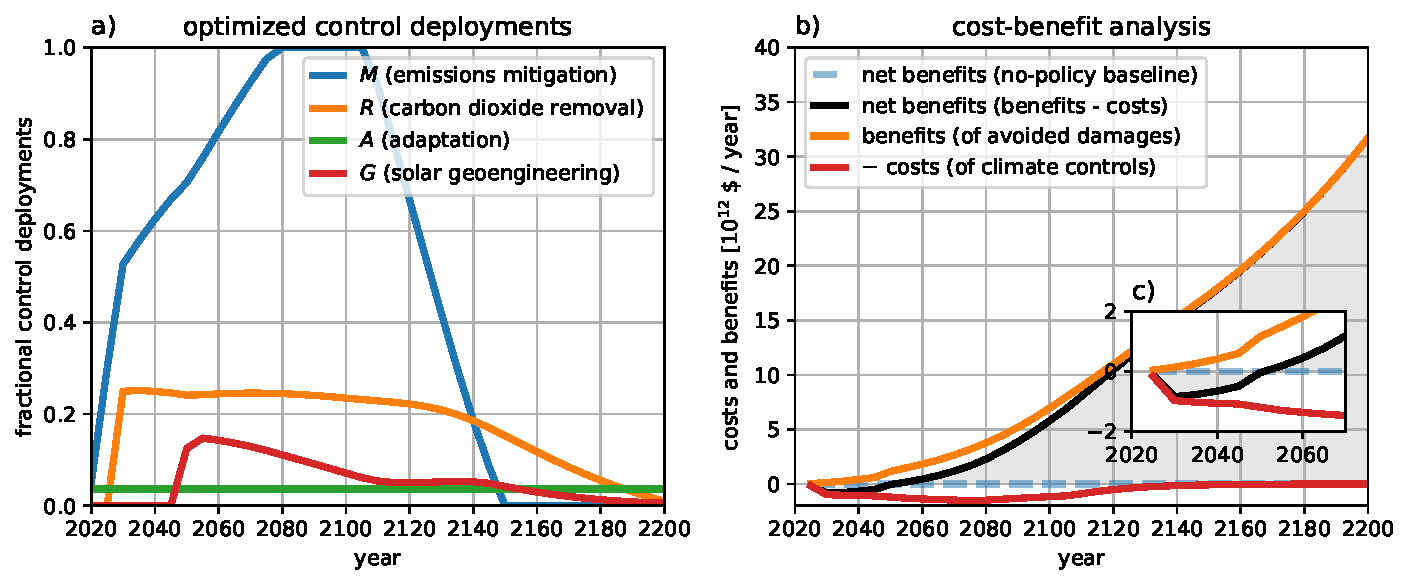
\includegraphics[width=1.0\textwidth]{figures/default-benefits_controls_and_benefits.pdf}
\centering
\caption{a) Optimal control deployments in a net benefit-maximizing framework and b) corresponding discounted costs and benefits relative to a no-climate-policy baseline scenario. The total positive area shaded in grey in b) is the maximal net present benefits (eq. \ref{eq.net_present_benefits}).}
\label{fig.approach1}
\end{figure}

\subsection{Approach 2: Cost-effectivness of avoiding damage thresholds}\label{sec.cost-effectivness}

In the cost-effectiveness framework, we aim to keep the adapted temperature $T_{M,R,G,A}$ (equivalently, controlled climate damages) below a threshold level $T^{\star}$ at a minimum net present cost of deploying climate controls:
\begin{align}
    &\min \left\{ \int_{t_{0}}^{t_{f}} \mathcal{C}_{M, R, G, A}\, (1 + \rho)^{-(t-t_{0})} \, \text{d}t \right\}\label{eq.cost_effectiveness} \quad\quad \\
    \text{subject to }\quad
    &T_{M, R, G, A} < T^{\star}.
\end{align}
The results of optimizing the cost-effectiveness of controls that keep adapted temperatures below $T^{\star} = \SI{2}{\celsius}$ are shown in Figures \ref{fig.temp_and_carbon} and \ref{fig.approach2}. Fractional emissions mitigation increases proportional to the increase in baseline emissions, reaching $M=\SI{90}{\%}$ decarbonization by 2100, while carbon dioxide is removed at a roughly constant rate of $R q_{0} \approx \SI{1.5}{ppm/year}$ starting in 2030. Since the optimally-controlled temperatures that result from cost-benefit analysis are already lower than $T^{\star}$ (not shown), the optimal controls from cost-effectiveness are here less ambitious than for the cost-benefit analysis (Figure \ref{fig.approach2}a vs. Figure \ref{fig.approach1}a). As a consequence of relatively relaxed mitigation and carbon dioxide removal early on, small but non-negligible deployment of solar-geoengineering is used to shave off a few tenths of a degree of warming during its peak in the mid-22nd Century in order to meet the temperature goal (Figure \ref{fig.approach2}a and Figure \ref{fig.temp_and_carbon}c). Adaptation offsets only $A = \SI{5}{\%}$ of damages and plays a minor role because the other controls have already substantially reduced damages. Even after discounting, annual costs of control deployments peak in 2100, driven by nearly synchronous peaks in mitigation and carbon dioxide removal.

\begin{figure}[htb!]
\noindent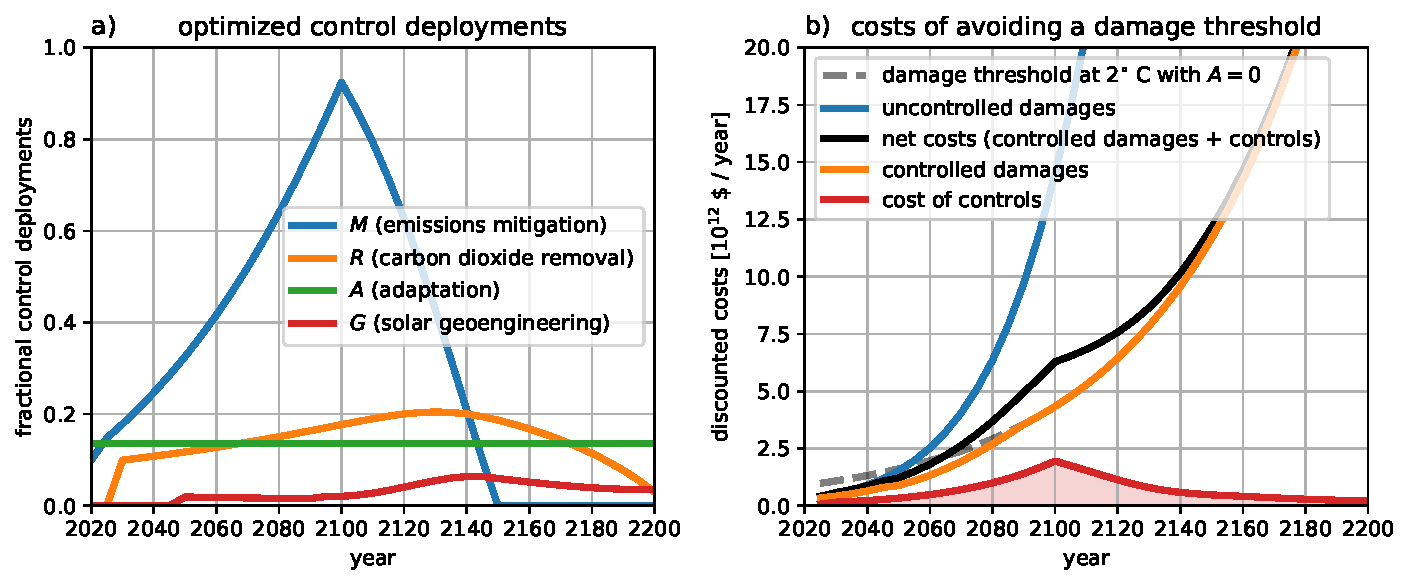
\includegraphics[width=1.0\textwidth]{figures/default-temp_controls_and_damages.pdf}
\centering
\caption{(a) Optimal control deployments in a net cost-effectiveness framework and (b) corresponding costs and damages. In panel (b), the blue line shows the discounted baseline uncontrolled damages; the dashed grey line shows the discounted damages associated with $2^{\circ}$ of warming which are to be avoided; the orange line shows the discounted damages in the optimally-controlled solution; and the red line shows the optimal discounted costs of controls such that the shaded area below is the minimal net present costs of controls (eq. \ref{eq.cost_effectiveness}).}
\label{fig.approach2}
\end{figure}

\section{Relative benefits of a complete portfolio of climate controls}
To quantify the benefits of considering a complete portfolio of climate controls, as opposed to considering control technologies in isolation, we compute optimal control trajectories with all $15$ combinations of the controls $\alpha \in \{M, A, R, G\}$, setting $\alpha \equiv 0$ for omitted technologies. Since considering an additional technology can only decrease the optimally-controlled costs and since there is no marginal cost for initial deployments, the most cost-effective strategy includes all four controls, with a net present cost of $55$ trillion USD. Since mitigation is the dominant control in the $\{MARG\}$ scenario, the eight most cost-effective portfolios include mitigation, with the mitigation-only $\{M\}$ scenario costing the most at a $66\%$ higher cost than the $\{MARG\}$ scenario (Table \ref{tab.relative_control_costs}). The costs of the remaining scenarios are much larger, with additional costs of $175\%$ for the all-but-mitigation scenario $\{ARG\}$ to $727\%$ for the solar geoengineering-only scenario $\{G\}$. In the adaptation-only scenario $\{A\}$, there is no solution that avoids an adapted temperature of $T^{\star} = \SI{2}{\celsius}$, because we have imposed adaptability limits $A < 1/3$. The existence of an interior global minimum that includes non-zero deployments of all four controls follows from the convexity of both the climate damage function and the control cost functions, and is not guaranteed under different forms of these poorly-constrained functions \citep[e.g.][]{lempert_multiple_2006}.

% policy action table
\begin{table}[t]
\begin{center}
 \begin{tabular}{|| c || c | c | c | c | c | c | c | c ||}
 \hline
 & MARG & MRG & MAR & MR & MAG & MG & MA & M \\ [0.5ex] 
 \hline
 Additional cost &
 0\% &
 2\% &
 9\% &
 11\% &
 38\% &
 42\% &
 58\% &
 62\%
 \\
 \hline\hline\hline
 & ARG & RG & AR & R & GA & G & A & \\
 \hline
 &
 175\% &
 207\% &
 305\% &
 372\% &
 524\% &
 727\% &
 N/A &
 \\
 \hline
 \end{tabular}
\end{center}
\caption{Additional net present cost of avoiding an adapted temperature of $T^{\star}=\SI{2}{\celsius}$, relative to the $55$ trillion USD net present cost of controls in the $\{MARG\}$ reference scenario with all four controls available: mitigation (M), adaptation (A), carbon dioxide removal (R) and solar geoengineering (G). Since we have imposed an upper bound $A<1/3$ on how much damage can be abated by adaptation, there is no scenario in which adaptation alone can keep damages below those associated with $T^{\star} = \SI{2}{\celsius}$ of warming.}
\label{tab.relative_control_costs}
\end{table}

\section{A policy process for responding to uncertain future outcomes}\label{sec.reactive}

Integrated Assessment Model (IAM) approaches, whether deterministic or stochastic, assume perfect foreknowledge of model dynamics, parameters (or their distributions), and inputs. Future outcomes will differ from projections because the models are imperfect approximations of the socio-economic and physical climate systems they represent. For example, socio-economic models may assume erroneous future costs of climate controls and physical climate models may omit tipping elements \citep{steffen_trajectories_2018}, both of which would lead to biases in model projections with respect to actual outcomes. Furthermore, the assumption of perfect foreknowledge degrades the active role of policy decision-makers and climate researchers in shaping the evolving distribution of model parameters. For example, developing control technology R\&D programs could bring down the future costs of controls faster than anticipated and new developments in climate science may cause estimates of physical parameter values to change over time.

% Prescribing fixed parameter values amounts to assuming perfect knowledge of socio-technological and physical climate systems with deep uncertainties and harboring disruptive surprises \citep{alley_abrupt_2003, steffen_trajectories_2018}.

A hypothetical empowered climate policy decision-maker must be in a position to respond to the inevitable differences that arise between model projections and actual outcomes and to revise their system understanding based on the newest developments in research. We show how our model equips climate policy decision-makers with the ability to periodically re-evaluate policy prescriptions by revising the underlying model structure and parameter values to correct for revealed biases.

The responsive control strategy process we propose is as follows:
\begin{enumerate}
    \item Initial future trajectories of optimal control deployments are computed from the vantage point of $t=t_{0}$;
    \item Model projections and control deployments are integrated forward one policy-making period to $t_{1}=t_{0} + \Delta t$;
    \item Model structure and parameter values are revised, owing to new information;
    \item Future trajectories of control deployments are re-optimized, now from the vantage point of $t_{1}=t_{0}+\Delta t$ and with revised model parameters;
    \item Return to step 2, replacing $t_{1} = t_{0} + \Delta t$ with $t_{n} = t_{n-1}+\Delta t$ for period $n$, and repeat the process for the desired number of periods.
\end{enumerate}

To illustrate the utility of the policy response process, we apply it to three hypothetical future scenarios, in which the most cost-effective control trajectories for keeping adapted temperatures below $T^{\star} = \SI{2}{\celsius}$ are sequentially re-optimized in response to changes in model inputs and parameters.

%Application of the framework is illustrated in three heuristic scenarios below, but could be more formally implemented in a Bayesian framework in which observations of the system over the period $\Delta t$ are used to update the prior parameter distributions to yield posterior parameter distributions which can be used to sequentially optimize the climate change trajectory.

\paragraph{Responding to variability in baseline emissions.}
Suppose in $t_{0} = 2020$ that the policy decision-maker prescribes aggressive climate policies (step 1), which are implemented such that future climate control deployments follow the optimally cost-effective trajectory for keeping warming below $T^{\star} = \SI{2}{\celsius}$ (step 2), as described in Section \ref{sec.cost-effectivness} (Figure \ref{fig.policy_updates}a, b). 

The policy decision-maker instructs a re-evaluation of the optimal control strategy at $t_{1} = 2050$, $\Delta t = 30$ years later. The actual baseline emission trajectory between $t_{0}=2020$ and $t_{1}=2050$ is found to be $r\Delta q = \SI{1}{ppm/year}$ higher than projected, resulting in higher CO$_{2e}$ concentrations than anticipated and warming that overshoots the $T^{\star} = \SI{2}{\celsius}$ goal by $\SI{0.12}{\celsius}$. The model inputs are thus revised to account for these higher-than-expected historical baseline emissions (step 3) and the optimal future control trajectories are re-computed (step 4), requiring an additional $\Delta M = \SI{2}{\%}$ to $\SI{4}{\%}$ of mitigation between $t_{1} = 2050$ and $2120$ (Figure \ref{fig.policy_updates}c), carrying an additional net present cost of $4$ trillion USD.

Suppose that, after following the re-optimized control trajectories for another $\Delta t = \SI{30}{years}$ (step 5), the historical effective baseline emissions must be revised downwards by $\SI{2.5}{ppm/year}$. This would imply a larger remaining carbon budget \citep{millar_cumulative_2016} and allows the policy decision-maker to relax control deployments while remaining below $T^{\star} = \SI{2}{\celsius}$ of warming (Figure \ref{fig.policy_updates}d), resulting in $10$ trillion USD of avoided net present costs of control deployments

\paragraph{Responding to under-estimation of geoengineering costs.}

Suppose that at a re-evaluation in 2050, carbon dioxide removal is $\SI{50}{\%}$ more expensive than projected. The climate policy-maker directs deployment of the most cost-effective control trajectories which keep warming below $T^{\star}=\SI{2}{\celsius}$, which are re-optimized with the revised cost of carbon dioxide removal. The result is to decrease carbon dioxide removal by $\Delta R = \SI{-5}{\%}$ and increase mitigation by $\Delta M = \SI{5}{\%}$, resulting in $2.5$ trillion USD of avoided net present costs of control deployments.

% Suppose that by $t = 2050$ it becomes clear that carbon dioxide removal at climate-relevant scales is $50\%$ more expensive than expected. The most cost-effective way forward would be to decrease carbon dioxide removal by $\Delta R = \SI{-5}{\%}$ and replace it by a corresponding increase in mitigation of $\Delta M = \SI{5}{\%}$ (Figure \ref{fig.policy_updates}e).

Suppose that after an additional \SI{30}{years}, during which solar geoenengineering is ramped up to $G=\SI{5}{\%}$, it becomes clear that the costs of unintended side-effects of solar geoengineering are four times larger than expected. In this scenario, the optimal future trajectory is to reduce solar-geoengineering to $G \approx \SI{0}{\%}$ and introduce a rapid short-term increase in mitigation of $\Delta M = \SI{5}{\%}$ (Figure \ref{fig.policy_updates}f), resulting in $17$ trillion USD of avoided net present costs.

\paragraph{Responding to under-estimation of Equilibrium Climate Sensitivity.}
Suppose that by 2050, a dramatically improved suite of general circulation climate models robustly exhibits Equilibrium Climate Sensitivities of $ECS=\SI{3.5}{\celsius}$, up from $\SI{3}{\celsius}$ in recent years \citep{geoffroy_transient_2012}, and further improvements result in $ECS=\SI{4}{\celsius}$ by 2080. Each of these revisions effectively shrinks the remaining cumulative carbon budget and thus require sequentially increased deployments of mitigation in order to keep warming below $T^{\star} = \SI{2}{\celsius}$ (Figures \ref{fig.policy_updates}g, h). Enough warming is already ``in the pipeline" by the second re-evaluation in 2080 that warming overshoots the $T^{\star} = \SI{2}{\celsius}$ goal and no solution exists unless the constraint is relaxed to $T^{\star} \geq \SI{2.08}{\celsius}$.

This section demonstrates it is possible to define a policy response process that permits a climate policy decision-maker to make successive adjustments to climate control strategies based on evolving outcomes and research developments. A disciplined response process thus simultaneously reaps the benefits of early action and minimizes the potential for regret by periodically adjusting for revealed policy or model deficiencies.

\begin{figure}[htb!]
\noindent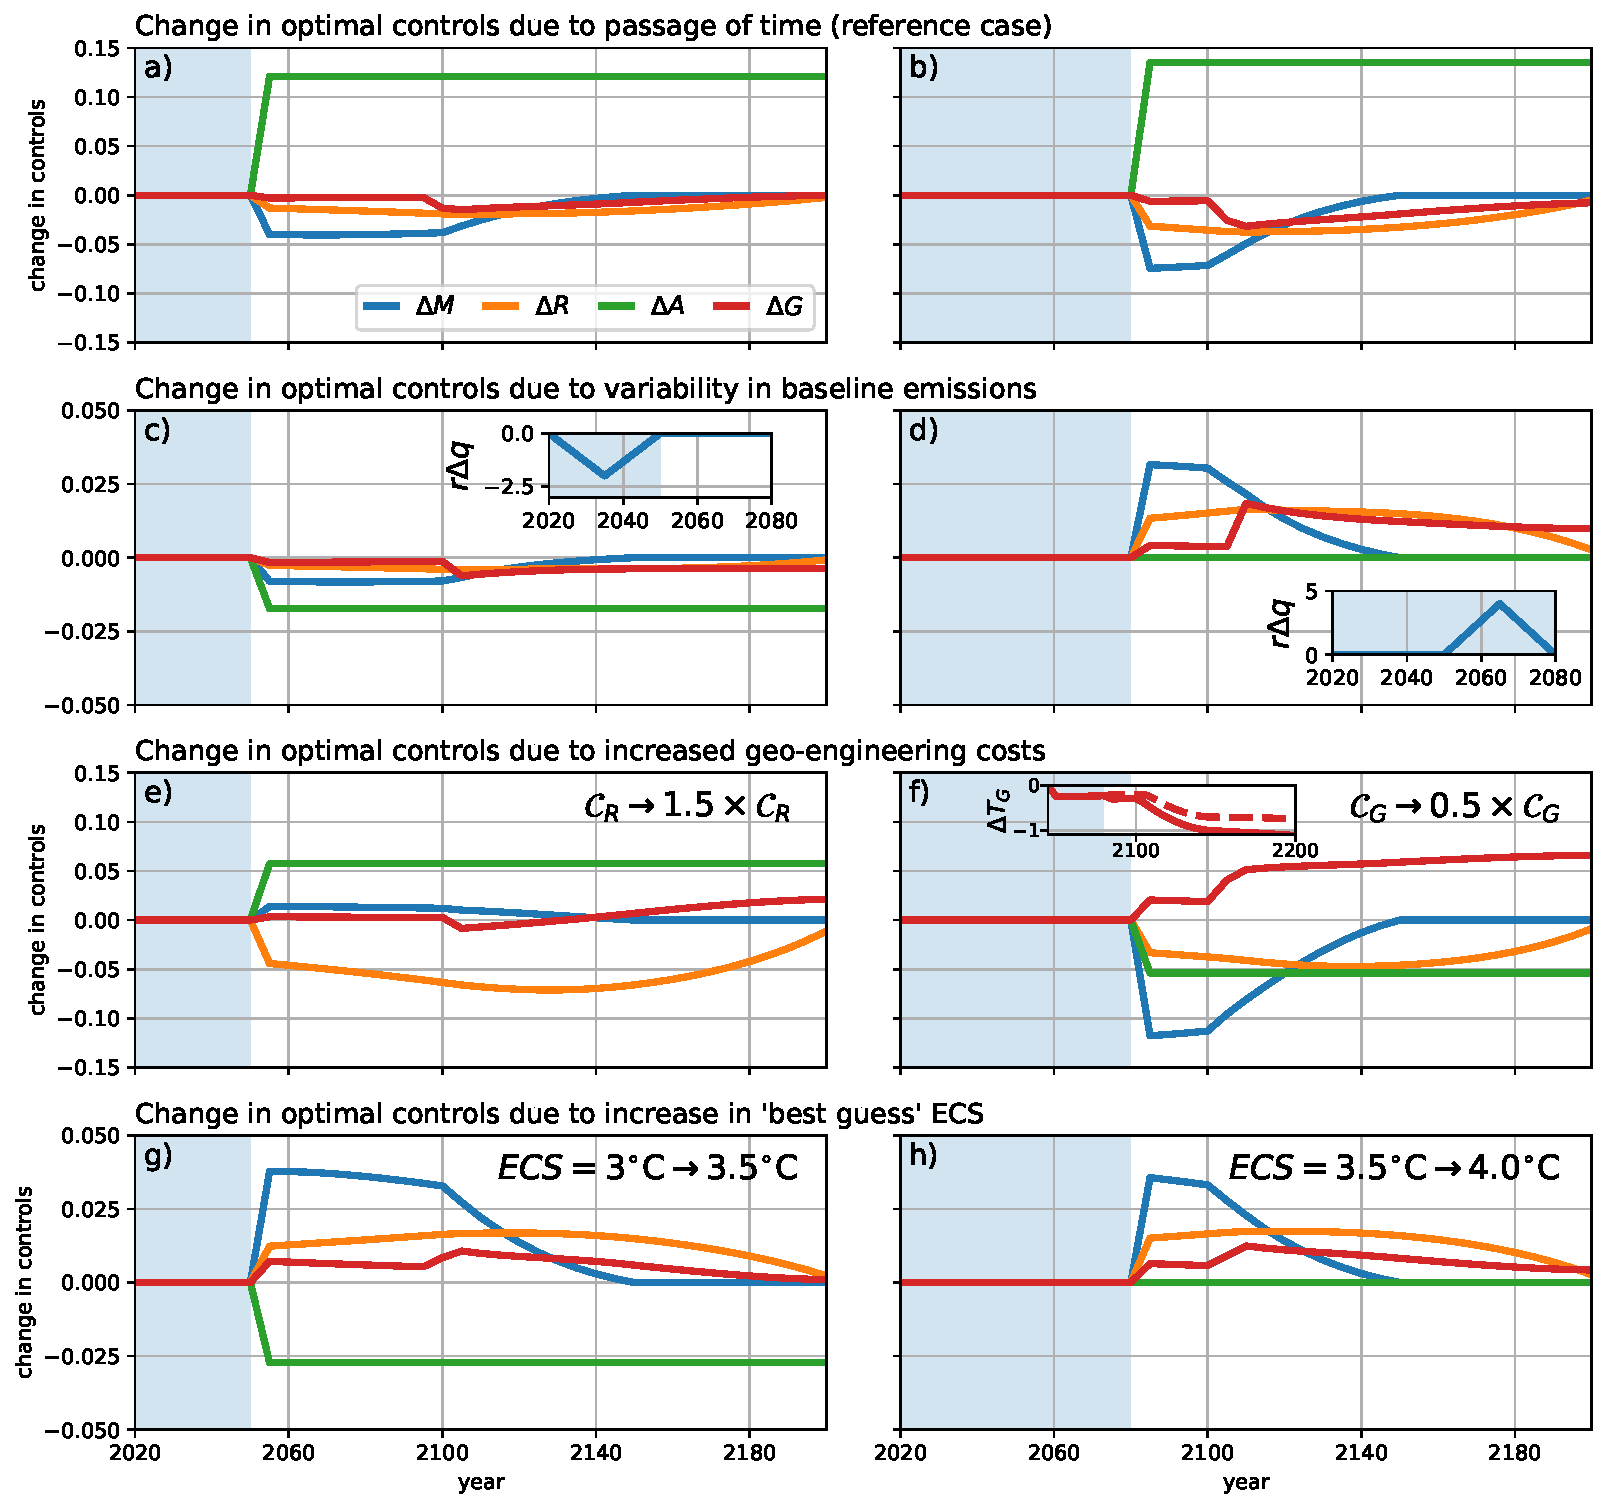
\includegraphics[width=0.925\textwidth]{figures/policy_updates.pdf}
\centering
\caption{Illustration of a proposed responsive policy progress. (a) Optimal climate control trajectories for avoiding $T^{\star} = \SI{2}{\celsius}$ of warming, as in Figure \ref{fig.approach2}a. (b) Baseline and optimally-controlled effective emissions, as well as the hypothetical variability in baseline emissions considered. (c-h) Difference in optimal control trajectories due to sequential re-optimization at 2050 and 2080 with revised model parameters: (c,d) where historical effective emissions $rq(t)$ are sequentially increased and then decreased (as shown in insets and in panel b), (e,f) where the costs of carbon and solar geo-engineering are sequentially increased, and (g,h) where the best guess of the Equilibrium Climate Sensitivity (ECS) is revised upwards in 2050 and again in 2080.}
\label{fig.policy_updates}
\end{figure}

% \section{Qualitative model results}

% \subsection{Extreme sensitivity to value-dependent discount rates}

% \subsection{Early mitigation minimizes the likelihood of regrets}

% \subsection{Multiple climate controls are better than one}

%\subsection{Uncertainty in climate damages strengthens the case for early action}

\section{Discussion}

Coming soon.

% \appendix
% \appendixpage
% \addappheadtotoc

%\section{Comprehensive formulation of optimization problems}

% \section{Justification and interpretation of free parameter values}\label{app.parameters}

% \subsection{Physical climate parameters}
% The temperature anomaly in $t_{0}=2020$ relative to pre-industrial is roughly $T_{0} = \SI{1.1}{\celsius}$, as estimated from a global network of in-situ thermometers \citep{lenssen_improvements_2019, nasagisstemp}.

% Present day CO$_{2e}(t_{0})$

% The free parameters in the two-box energy balance model are set by the multi-model mean values diagnosed from the CMIP5 ensemble of general circulation climate models by \cite{geoffroy_transient_2012} (Tables 3 and 4). They are: the deep ocean heat capacity $C_{D} (\equiv C_{0}$), the heat exchange coefficient $\kappa (\equiv \gamma)$, and the feedback parameter $B (\equiv \lambda)$. These values are more easily interpreted with the following diagnostic variables: the Transient Climate Sensivity $TCS = \Delta F_{2\times}/(B + \kappa)$, the warming that arises shortly after a doubling of CO$_{2}$ concentrations; the Equilibrium Climate Sensitivity $ECS = \Delta F_{2\times}/B$, the equilibrium temperature anomaly due to a doubling of CO$_{2}$ concentrations, and the ocean heat uptake timescale $\tau_{D}$ which controls the asymptotic approach to the equilibrium temperature.

% \subsection{Economic model parameters}
% In the face of habitability limits \citep[e.g.][]{sherwood_adaptability_2010} and exorbitant adaptation costs at high levels of warming, some unknown fraction of climate damages cannot be avoided by adaptation \citep{chambwera2014economics}; here, we impose this constraint somewhat arbitrarily by setting $0 \le A \le 1/3$. We base our reference cost for adaptation  $\mathcal{C}_{A}$ on \cite{agr2018}, which estimates annual adaptation costs of $\SI{500}{billion\; USD2010\; yr^{-1}}$ by 2050. We assume that the \cite{agr2018} adaptation reflects the cost of offsetting $A = 1/3$ of climate damages and thus set $\mathcal{C}_{A} (1/3)^{2} = \SI{500}{billion\; USD2010\; yr^{-1}}$ or $\mathcal{C}_{A} = \SI{4.5}{trillion\; USD2010\; yr^{-1}}$.

% \section{Replication of qualitative results from other models}\label{app.replication}

% policy action table
\subsection{Policy action parameters}
\begin{table}[t]
\begin{center}
 \begin{tabular}{|| c || c ||}
 \hline
 Parameter & Default Configuration \\ [0.5ex] 
 \hline\hline
 $t_{0}$ & 2020 \\
 \hline
 $t_{f}$ & 2200 \\
 \hline
 $\delta t$ & \SI{5}{yr} \\
 \hline
 $c_{0}$ & \SI{460}{ppm} \\ 
 \hline
 a & \SI{4.97}{W m^{-2}}\\
 \hline
 $q(t)$ & See eq. (\ref{eq.baseline_emissions}) \\
 \hline
 $r$ & $40\%$ \\
 \hline
 $T_{0}$ & \SI{1.1}{K} \\
 \hline
 $B$ & \SI{1.13}{W\, m^{-2}\, K^{-1}} \\
 \hline
 $\kappa$ & \SI{0.72}{W\, m^{-2}\, K^{-1}} \\
 \hline
 $C_{D}$ & \SI{106}{W\, yr\, m^{-2}\, K^{-1}} \\
 \hline
 $\beta$ & \SI{0.22e12}{\$\, yr^{-1}\, K^{-2}} \\
 \hline
 $\rho$ & $1\%$ \\
 \hline
 $E_{0}$ & \SI{100e12}{\$\, yr^{-1}}\\
 \hline
 $\gamma$ & $2\%$ \\
 \hline\hline
 \end{tabular}
\end{center}
\caption{}
\label{tab.parameters}
\end{table}

% Control parameter table
\begin{table}[t]
\begin{center}
 \begin{tabular}{|| c || c ||}
 \hline
 Parameter & Default Configuration \\ [0.5ex] 
 \hline\hline
 $M$ & $0 \le M \le 1$ \\
 \hline
 $A$ & $0 \le A \le 1/3$ \\
 \hline
 $R$ & $0 \le R \le 1$ \\
 \hline
 $G$ & $0 \le G \le 1$ \\
 \hline
 $\dot{M}$ & \SI{1/20}{yr^{-1}} \\
 \hline 
 $\dot{A}$ & \SI{0}{yr^{-1}} \\
 \hline 
 $\dot{R}$ & \SI{1/20}{yr^{-1}} \\
 \hline 
 $\dot{G}$ & \SI{1/20}{yr^{-1}} \\
 \hline 
 $t_{M}$ & $2020$ \\
 \hline
 $t_{A}$ & $2020$ \\
 \hline
 $t_{R}$ & $2030$ \\
 \hline
 $t_{G}$ & $2050$ \\
 \hline
 $M_{0}$ & $\SI{5}{\%}$ \\
 \hline
 $A_{0}$ & $0$ \\
 \hline
 $R_{0}$ & $0$ \\
 \hline
 $G_{0}$ & $0$ \\
 \hline
 \hline
 \hline
 $\mathcal{C}_{M}$ & \SI{2e12}{\$\, yr^{-1}} \\
 \hline
 $\mathcal{C}_{A}$ & \SI{4.5e12}{\$\, yr^{-1}} \\
 \hline
 $\mathcal{C}_{R}$ & \SI{8.3e12}{\$\, yr^{-1}} \\
 \hline
 $\tilde{\mathcal{C}}_{G}$ & \SI{4.6}{\percent} \\ 
 \hline
 $p_{M}$ & $2$ \\
 \hline
 $p_{A}$ & $2$ \\
 \hline 
 $p_{R}$ & $2$ \\
 \hline
 $p_{G}$ & $2$ \\
 \hline\hline
\end{tabular}
\end{center}
\caption{Values of parameters governing control variable constraints (above separation) and deployment costs (below separation).}
\label{tab.controls}
\end{table}

\bibliographystyle{apalike}
%\bibliographystyle{unsrtnat}
\bibliography{references.bib, refs_by_hand.bib}

\end{document}